\documentclass[border=10pt]{standalone}
\usepackage{pgfplots}
\usepackage{fontspec}
\setmainfont{Comic Sans MS}
\begin{document}
\definecolor{blue}{RGB}{31,119,180}
\pgfmathsetseed{1}
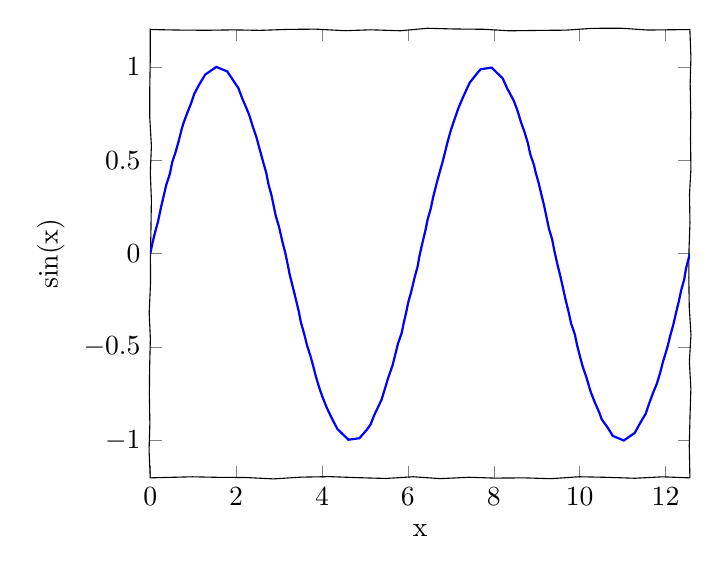
\begin{tikzpicture}[decoration={random steps, segment length=10pt,
                                amplitude=0.5pt}, decorate]
    \begin{axis}[xmin=0, xmax=4*pi, xlabel=x, ylabel=sin(x)]
        \begin{scope}[decoration={random steps, segment length=4pt,
                                  amplitude=0.2pt}, decorate]
            \addplot[domain=0:4*pi, samples=50, blue, thick] {sin(deg(x))};
        \end{scope}
    \end{axis}
\end{tikzpicture}
\end{document}
